\section{S-ENSO an index for a shifting warming patters}
We propose that the spatial distribution of Pacific Ocean warming might provide better predictive insights into ENSO-Atlantic TC activity relationship than warming anomalies alone. 
The S-ENSO index is computed by first averaging the SST anomalies over the June-October period to accurately capture ENSO's evolution prior to and during the Atlantic hurricane season (August-October). We then search the tropical Pacific ($5^\circ$S-$30^\circ$N) for a region of similar size than traditional ENSO indices that has the highest mean SST anomaly over the June-October period. %(see figure \ref{fig:s_enso_graphic}). 
We repeat this procedure for each year from 1979 to 2010. Table \ref{ref:lin_corr} shows S-ENSO's linear correlation coefficients with various quantities that communicate August-October Atlantic TC activity: number of tropical cyclones, number of major hurricanes, potential dissipation index (PDI) \cite{emanuel2005a}, accumulated cyclone energy (ACE) \cite{Bell2000}, and net tropical cyclone energy (NTC) \cite{goldenberg2001}. The significant improvement over traditional static NINO indices, especially with regards to cumulative statistics such as ACE and NTC indicates that S-ENSO is better at resolving the large-scale conditions over the Atlantic.

\begin{table}
\begin{tabular}{cccccc}
\hline
&TCs & Major Hurricanes & NTC & PDI & ACE\\
\hline
%S-ENSO  & \textbf{0.81} & \textbf{0.81} & \textbf{0.77} & \textbf{0.71} & \textbf{0.75}\\
%PWP-Pres & 0.61 & 0.65 & 0.57 & 0.56 & 0.58\\
%PWP-OLR & 0.55 & 0.57 & 0.50 & 0.46 & 0.48\\
%MinPres-Lon & 0.15 & 0.12 & 0.19 & 0.17 & 0.20\\
%PWP-PCP  & 0.67 & 0.66 & 0.64 & 0.6 & 0.58\\
%maxSSTALon & \textbf{-0.64} & -0.5 & \textbf{-0.55} & -0.44 & \textbf{-0.49}\\
S-ENSO & \textbf{-0.75} & \textbf{-0.59} &\textbf{-0.74} & \textbf{-0.68} & \textbf{-0.73}\\
Nino1+2 & -0.51 & -0.46 & -0.46 & -0.4 & -0.42\\
Nino 3 & -0.51 & -0.51 & -0.48 & -0.44 & -0.45\\
Nino 4 & -0.32 & -0.47 & -0.32 & -0.3 & -0.31\\
Nino 3.4 & -0.47 & -0.53 & -0.46 & -0.43 & -0.45\\
%Modoki Box A & -0.28 & -0 & -0.26 & -0.24 & -0.3\\
%Modoki Box B & -0.41 & -0.40 & -0.4 & -0 & -0.33\\
%Modoki Box C & 0.55 & 0.57 & 0.57 & 0.57 & 0.59\\
%Modoki EMI & -0.062 & -0.21 & -0.088 & -0.11 & -0.12\\
\hline
\end{tabular}
\caption{Linear correlation coefficients between the June-October S-ENSO and August-October Atlantic TC activity. The highest score for each category is highlighted in \textbf{bold}. All correlations are significant at $95\%$ level}
\label{ref:lin_corr}
\end{table}

In addition to providing better in-season accuracy than traditional NINO indices, S-ENSO is more robust to the ENSO spring predictability barrier \cite{webster1992}. Figure \ref{fig:figures_lead_time_bar} shows the performance of each NINO index as well as S-ENSO as a function of lead time. While S-ENSO's performance drops with January lead time, it is nearly an order of magnitude better than that of some static NINO indices. If dynamical models can resolve the spatial patterns of ENSO as represented by S-ENSO then dynamical models could potentially have significant skill in predicting August-October TC activity.

\begin{figure}[htbp]
	\centering
		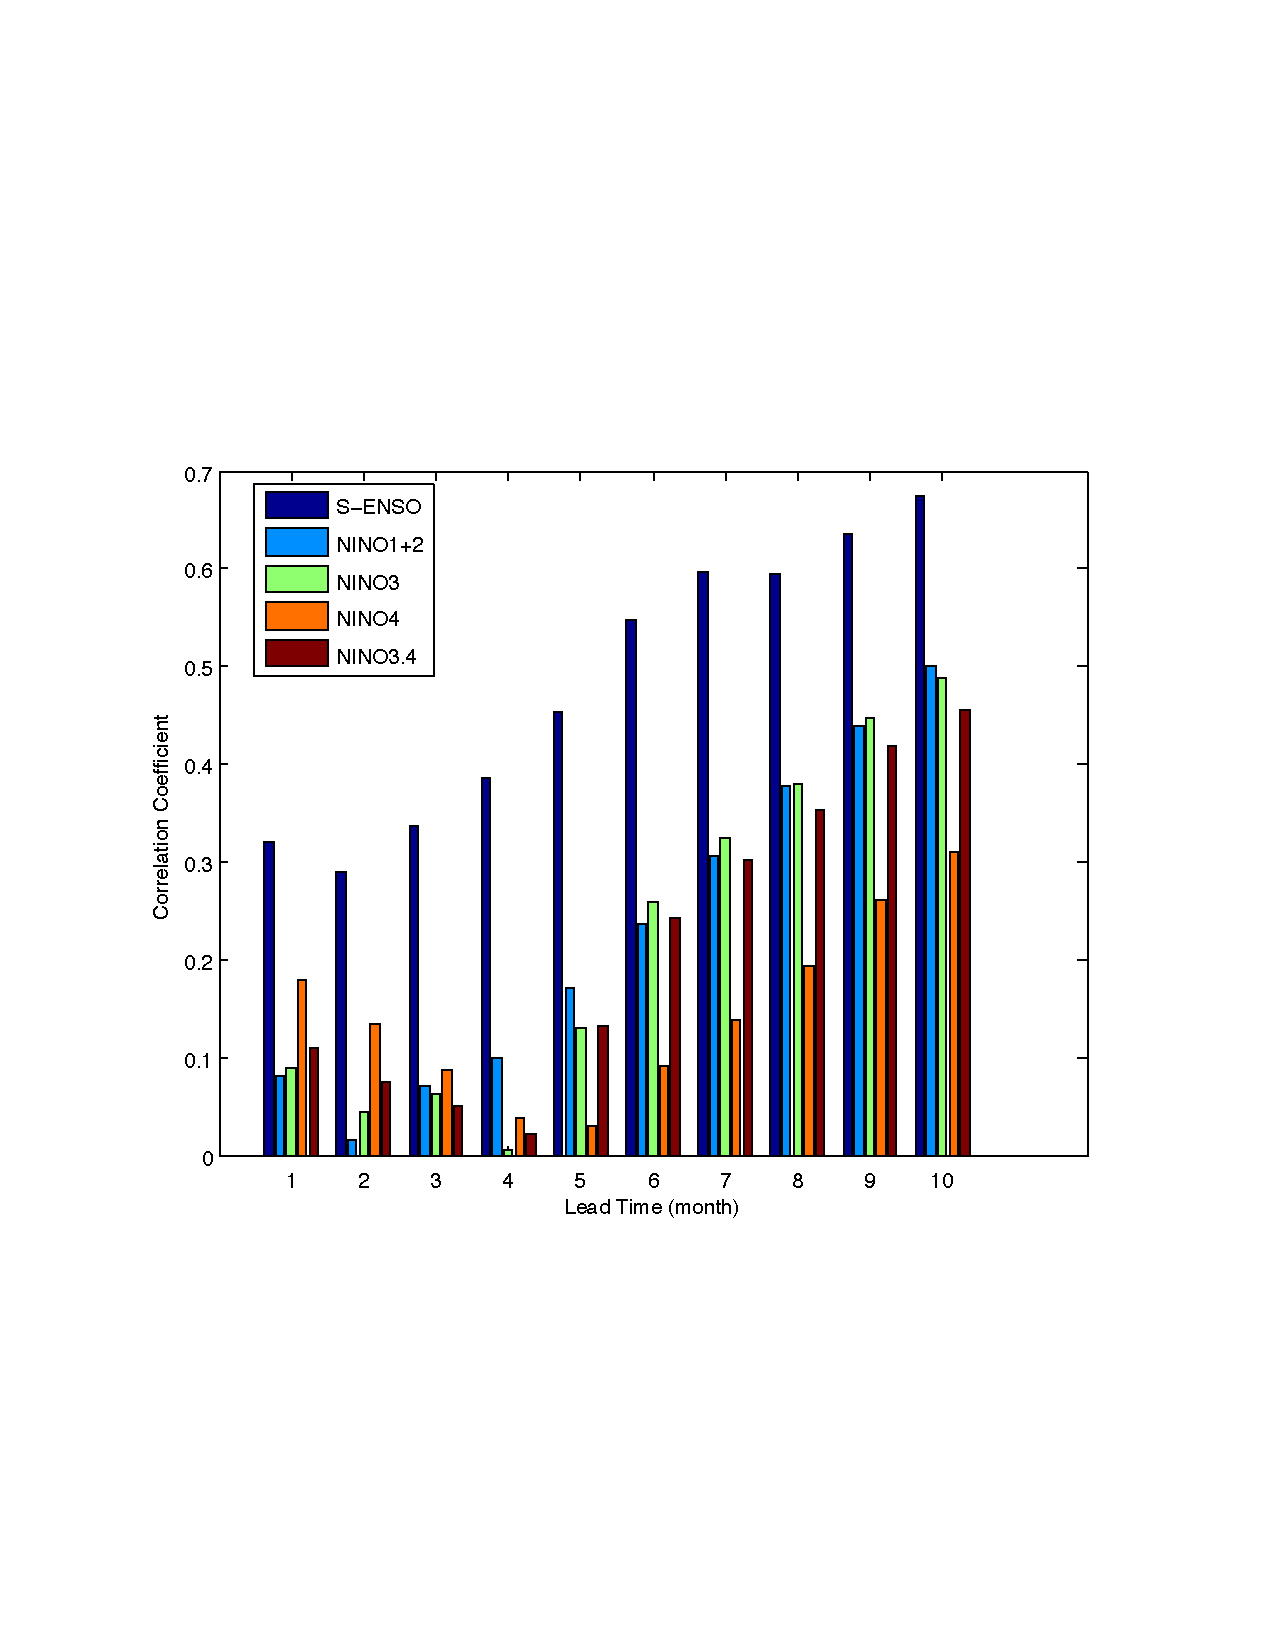
\includegraphics[height=3in]{figures/lead_time_bar.pdf}
	\caption{The linear correlation coefficients between different ENSO indices and Atlantic August-October TC counts. The y-axis denotes the last month used to build the index. The indices increase in accuracy as we move closer to the TC season, however S-ENSO performance is not as severely affected by the ENSO predictability barrier as traditional NINO indices.}
	\label{fig:figures_lead_time_bar}
\end{figure}

\newpage
